\documentclass[11pt,]{article}
\usepackage[left=1in,top=1in,right=1in,bottom=1in]{geometry}
\newcommand*{\authorfont}{\fontfamily{phv}\selectfont}
\usepackage[]{mathpazo}


  \usepackage[T1]{fontenc}
  \usepackage[utf8]{inputenc}



\usepackage{abstract}
\renewcommand{\abstractname}{}    % clear the title
\renewcommand{\absnamepos}{empty} % originally center

\renewenvironment{abstract}
 {{%
    \setlength{\leftmargin}{0mm}
    \setlength{\rightmargin}{\leftmargin}%
  }%
  \relax}
 {\endlist}

\makeatletter
\def\@maketitle{%
  \newpage
%  \null
%  \vskip 2em%
%  \begin{center}%
  \let \footnote \thanks
    {\fontsize{18}{20}\selectfont\raggedright  \setlength{\parindent}{0pt} \@title \par}%
}
%\fi
\makeatother




\setcounter{secnumdepth}{3}

\usepackage{longtable,booktabs}

\usepackage{graphicx,grffile}
\makeatletter
\def\maxwidth{\ifdim\Gin@nat@width>\linewidth\linewidth\else\Gin@nat@width\fi}
\def\maxheight{\ifdim\Gin@nat@height>\textheight\textheight\else\Gin@nat@height\fi}
\makeatother
% Scale images if necessary, so that they will not overflow the page
% margins by default, and it is still possible to overwrite the defaults
% using explicit options in \includegraphics[width, height, ...]{}
\setkeys{Gin}{width=\maxwidth,height=\maxheight,keepaspectratio}

\title{Patrones de Asociación y Diversidad Descritos por la Familia Fabaceae
Mimosoideae en una Isla Subtropical, Cuenca del Mar Caribe.\\
\emph{Patterns of Association and Diversity Described by the Family
Fabaceae Mimosoideae on a Subtropical Island, Caribbean Sea Basin}.\\  }



\author{\Large Welifer Junior Lebron Vicente\vspace{0.05in} \newline\normalsize\emph{Estudiante de Ciencias Geográficas, Universidad Autónoma de Santo
Domingo (UASD)}  }


\date{}

\usepackage{titlesec}

\titleformat*{\section}{\normalsize\bfseries}
\titleformat*{\subsection}{\normalsize\itshape}
\titleformat*{\subsubsection}{\normalsize\itshape}
\titleformat*{\paragraph}{\normalsize\itshape}
\titleformat*{\subparagraph}{\normalsize\itshape}

\titlespacing{\section}
{0pt}{36pt}{0pt}
\titlespacing{\subsection}
{0pt}{36pt}{0pt}
\titlespacing{\subsubsection}
{0pt}{36pt}{0pt}





\newtheorem{hypothesis}{Hypothesis}
\usepackage{setspace}

\makeatletter
\@ifpackageloaded{hyperref}{}{%
\ifxetex
  \PassOptionsToPackage{hyphens}{url}\usepackage[setpagesize=false, % page size defined by xetex
              unicode=false, % unicode breaks when used with xetex
              xetex]{hyperref}
\else
  \PassOptionsToPackage{hyphens}{url}\usepackage[unicode=true]{hyperref}
\fi
}

\@ifpackageloaded{color}{
    \PassOptionsToPackage{usenames,dvipsnames}{color}
}{%
    \usepackage[usenames,dvipsnames]{color}
}
\makeatother
\hypersetup{breaklinks=true,
            bookmarks=true,
            pdfauthor={Welifer Junior Lebron Vicente (Estudiante de Ciencias Geográficas, Universidad Autónoma de Santo
Domingo (UASD))},
             pdfkeywords = {palabra clave 1, palabra clave 2},  
            pdftitle={Patrones de Asociación y Diversidad Descritos por la Familia Fabaceae
Mimosoideae en una Isla Subtropical, Cuenca del Mar Caribe.\\
\emph{Patterns of Association and Diversity Described by the Family
Fabaceae Mimosoideae on a Subtropical Island, Caribbean Sea Basin}.\\},
            colorlinks=true,
            citecolor=blue,
            urlcolor=blue,
            linkcolor=magenta,
            pdfborder={0 0 0}}
\urlstyle{same}  % don't use monospace font for urls

% set default figure placement to htbp
\makeatletter
\def\fps@figure{htbp}
\makeatother

\usepackage{pdflscape} \newcommand{\blandscape}{\begin{landscape}}
\newcommand{\elandscape}{\end{landscape}}


% add tightlist ----------
\providecommand{\tightlist}{%
\setlength{\itemsep}{0pt}\setlength{\parskip}{0pt}}

\begin{document}
	
% \pagenumbering{arabic}% resets `page` counter to 1 
%
% \maketitle

{% \usefont{T1}{pnc}{m}{n}
\setlength{\parindent}{0pt}
\thispagestyle{plain}
{\fontsize{18}{20}\selectfont\raggedright 
\maketitle  % title \par  

}

{
   \vskip 13.5pt\relax \normalsize\fontsize{11}{12} 
\textbf{\authorfont Welifer Junior Lebron Vicente} \hskip 15pt \emph{\small Estudiante de Ciencias Geográficas, Universidad Autónoma de Santo
Domingo (UASD)}   

}

}








\begin{abstract}

    \hbox{\vrule height .2pt width 39.14pc}

    \vskip 8.5pt % \small 

\noindent Mi resumen


\vskip 8.5pt \noindent \emph{Keywords}: palabra clave 1, palabra clave 2 \par

    \hbox{\vrule height .2pt width 39.14pc}



\end{abstract}


\vskip 6.5pt


\noindent  \section{Introducción}\label{introducciuxf3n}

El análisis de biodiversidad forestal viabiliza la obtención de
información sobre el comportamiento de las especies en su hábitat, los
efectos de cambios geoestacionarios, y las probables consecuencias de
actividades antrópicas en el ciclo vital de los bosques. La función de
los bosques tropicales puede ser productiva (madera, fibra, leña,
productos no maderables); ambientales (regulación del clima, reserva de
biodiversidad, conservación de suelos y agua, etc.); y social
(subsitencia de poblamientos humanos locales y su cultura) (Montagnini,
Jordan, \& others, 2005).

Montagnini et al. (2005) La isla Barro Colorado, de coordenadas {[}9º 9'
0'`N, 79º 51' 0'' W{]}, es una plataforma basáltica miocénica sobre la
que descansa un bosque tropical primario compuesto por 305 especies
arboreas {[}cita2,C. article{]}. En el período 1981-2015 fue el
emplazamiento de ocho censos forestales realizados por el Smithsonian
Tropical Research Institute, donde la subfamilia \emph{Fabaceae
Mimosoideae} representa el 5.9\% de las especies registradas en la
parcela de 50 hectareas delimitada en 1980 {[}Cita3,WebP{]}.

\begin{figure}
\centering
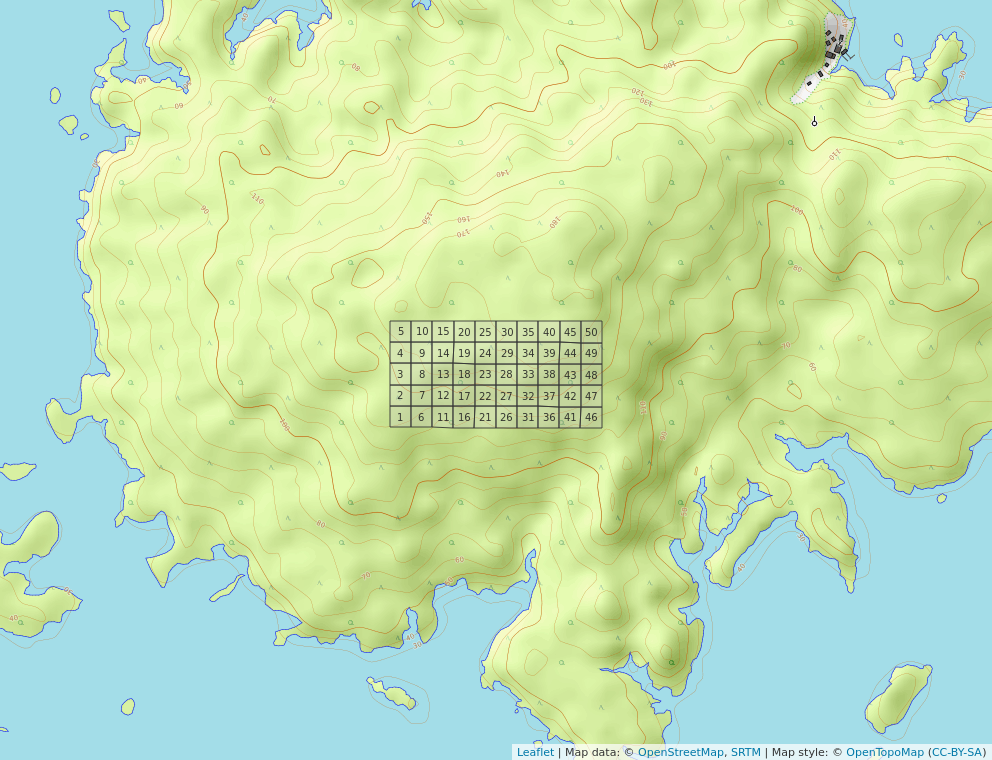
\includegraphics[width=0.50000\textwidth]{mapa_cuadros.png}
\caption{Área del censo forestal, Barro Colorado Island (1981-2015).}
\end{figure}

La familia \emph{Mimosoideae} fue incorporada a las
\emph{Caesalpinoideae} dentro del clado mimosoide, esta subfamilia de
las fabaceas es sumamente variable; compuesta principalmente por árboles
y arbustos de flores asimétricas cigomorfas. El clado filogenético
mimosoide es propio de climas tropicales y subtropicales, sus flores son
simétricas con petalos valvados y sus especimenes tienen un gran número
de estambres prominentes. {[}Cita \#4{]} \ldots.

\section{Metodología}\label{metodologuxeda}

Se seleccionó la subfamilia \emph{Fabaceae Mimosoideae} dentro del total
de 59 familias censadas por el Smithsonian Tropical Research Institute
en una parcela de 50 hectareas en la isla Barro Colorado. \ldots

\section{Resultados}\label{resultados}

(ver tabla \ref{tab:abun_sp} y figura \ref{fig:abun_sp_q})

\begin{longtable}[]{@{}lr@{}}
\caption{\label{tab:abun_sp}Abundancia por especie de la familia
\emph{Fabaceae-Mimosoideae}.}\tabularnewline
\toprule
Latin & n\tabularnewline
\midrule
\endfirsthead
\toprule
Latin & n\tabularnewline
\midrule
\endhead
Inga marginata & 767\tabularnewline
Inga umbellifera & 765\tabularnewline
Inga acuminata & 606\tabularnewline
Inga nobilis & 557\tabularnewline
Inga goldmanii & 297\tabularnewline
Inga thibaudiana & 232\tabularnewline
Inga sapindoides & 197\tabularnewline
Inga pezizifera & 145\tabularnewline
Inga laurina & 57\tabularnewline
Inga punctata & 57\tabularnewline
Inga cocleensis & 54\tabularnewline
Acacia melanoceras & 48\tabularnewline
Inga spectabilis & 20\tabularnewline
Abarema macradenia & 19\tabularnewline
Enterolobium schomburgkii & 12\tabularnewline
Inga ruiziana & 8\tabularnewline
Inga oerstediana & 4\tabularnewline
Cojoba rufescens & 2\tabularnewline
\bottomrule
\end{longtable}

\begin{figure}
\centering
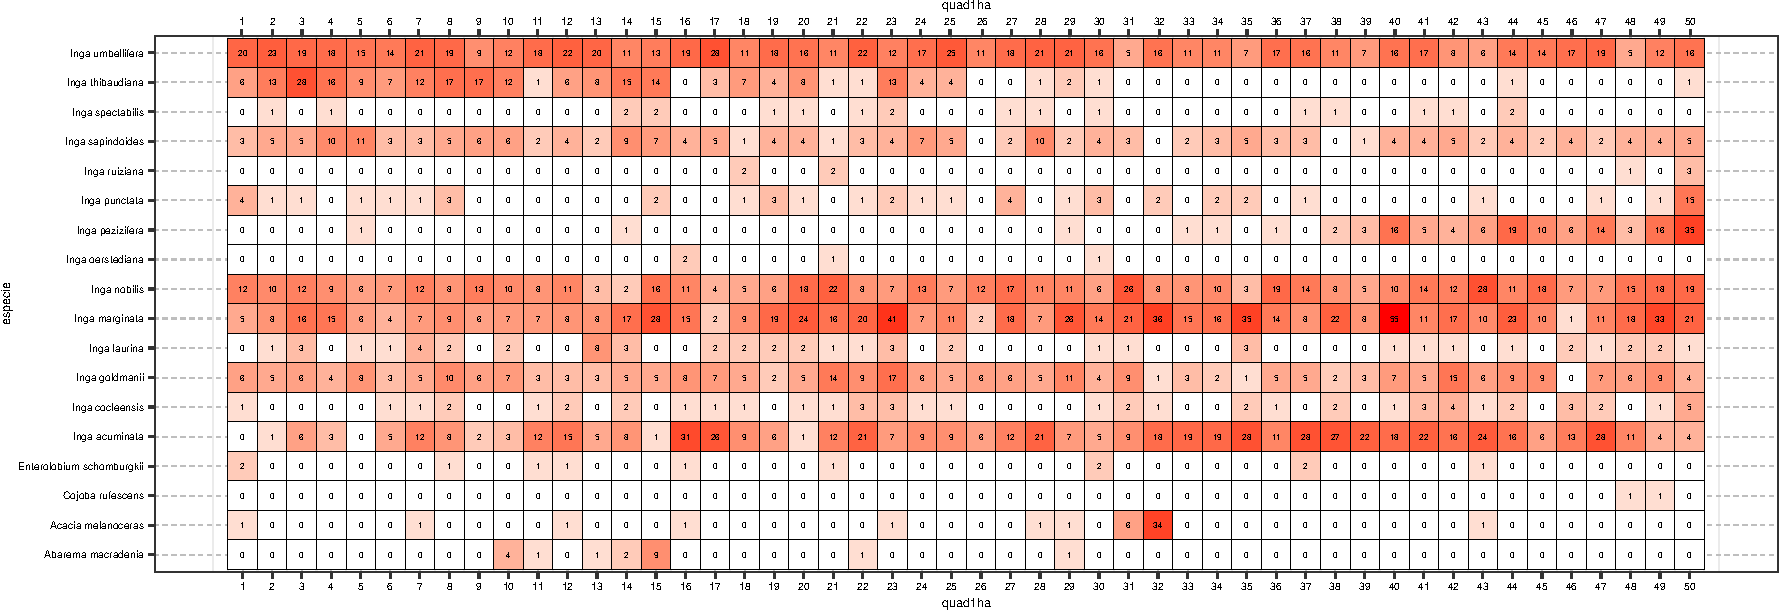
\includegraphics{manuscrito_files/figure-latex/unnamed-chunk-3-1.pdf}
\caption{\label{fig:abun_sp_q}Abundancia por especie por quadrat}
\end{figure}

\section{Discusión}\label{discusiuxf3n}

\section{Agradecimientos}\label{agradecimientos}

\section{Información de soporte}\label{informaciuxf3n-de-soporte}

\ldots

\section{\texorpdfstring{\emph{Script}
reproducible}{Script reproducible}}\label{script-reproducible}

\ldots

\section*{Referencias}\label{referencias}
\addcontentsline{toc}{section}{Referencias}

\hypertarget{refs}{}
\hypertarget{ref-montagnini2005tropical}{}
Montagnini, F., Jordan, C. F., \& others. (2005). \emph{Tropical forest
ecology: The basis for conservation and management}. Springer Science \&
Business Media.




\newpage
\singlespacing 
\end{document}
